The project case is at the core of the workflow since it acts as the interface between the AR- and VR-components of the workflow.

\begin{figure}[ht]
    \centering
    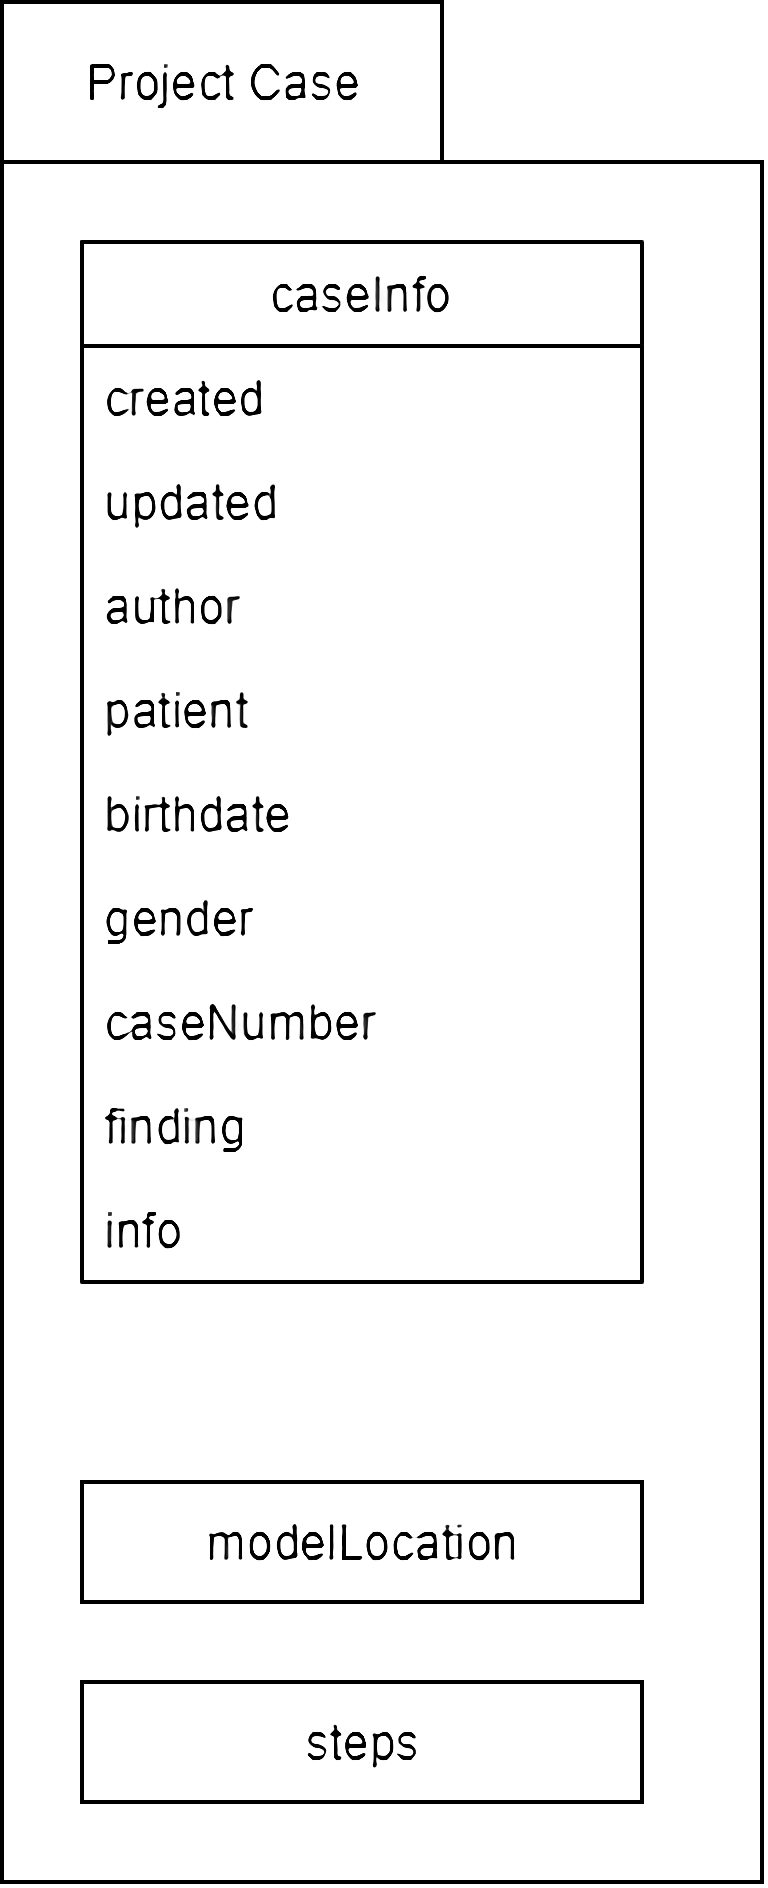
\includegraphics[width=110px]{images/implementation/project_case.png}
    \caption{\label{fig::ImplementationProjectCase}Structure of a Project Case}
\end{figure}

The specifics about the project case's JSON-notation are depicted in Figure \ref{fig::ImplementationProjectCase}.
The \emph{caseInfo} contains patient specific information which may be important for the procedure.
These informations, as well as the location of the patients 3D data on the hard drive, have to be manually input by users.
Information about the steps will be automatically generated while perfoming procedures inside of the application, however, users can then later add additional information as they see fit.
The automatically generated information about the steps only contains information about which instrument was used at which step of the procedure.

When a project case is saved from within the application, a copy of the current patient with all steps, which were performed is made withing the root folder of the patient model.
This way, the patient's model is never lost and the procedure can always be started from scratch if desired.
Also, the timestamp of the updated field inside of the caseInfo will be set.

By simply adding the planned procedures as additional 3D data to the patient, extensibility and robustness of the software are ensured.
New instruments and thus procedures can easily be added into the application without touching the project cases and everything will continue working as expected.
In comparison, if an approach where procedures have to be defined from within the project case was used, project cases would have to be updated every time new 
instruments are added to the application.